\documentclass[
    % -- opções da classe memoir --
    12pt,				% tamanho da fonte
    a4paper,            % tamanho do papel
    oneside,			% para impressão em recto e verso. Oposto a twoside
    openright,			% capítulos começam em pág ímpar (insere página vazia caso preciso)
    ruledheader,
    %noindentfirst,
    anapcustomindent,
    sumario = tradicional,
    abntfigtabnum,
    tocpage=plain,
    english,			% idioma adicional para hifenização
	%french,				% idioma adicional para hifenização
	%spanish,			% idioma adicional para hifenização
	brazil,				% o último idioma é o principal do documento
    ]{abntex-ifrn/abntex2-trabalho} % modificação no abnTeX2 para usar orientadora feminina, dentre outras alterações. Se for orientador realizar a alteração no arquivo.


% ---
% PACOTES IFSULDEMINAS
% ---
\usepackage{abntex-ifrn/abntex-ifrn} %estilo dos nomes dos capítulos e sumário conforme IFSULDEMINAS
%Estilo de formatação de capítulos, padrão IFSULDEMINAS

\makeatletter
\newcommand{\thechapterwords}
{ \ifcase \thechapter\or 1\or 2\or 3\or 4\or 5\or 6\or 7\or 8\or 9\or 10\or 11\fi} % se precisar de mais capítulos adicionar conforme a ordem lógica estabelecida.

\def\@makechapterhead#1{%
\vspace*{6cm} % insere o espaço de 6cm da margem, conforme estabelecido.
{\parindent \z@  \reset@font

\bfseries \thechapterwords.  #1\par\nobreak % AQUI ESTÁ O NOME DO CAPÍTULO
\par
\vspace*{10\p@}% pequeno espaçamento após o nome do capítulo
}}

\setsecheadstyle{}
\setsubsecheadstyle{}
\setsubsubsecheadstyle{}
\setparaheadstyle{}
\setsubparaheadstyle{} %modelos dos capítulos
% ---
% Pacotes fundamentais 
% ---
\usepackage{amsmath}
\usepackage{mathspec}
\setmainfont[Ligatures=TeX]{Times New Roman} %Pode ser Arial em ambos
\setsansfont[Ligatures=TeX]{Times New Roman}
\setmonofont{Times New Roman}
\setmathrm{Times New Roman}
\setmathfont(Digits,Latin){Times New Roman} % Fonte matemática Times

\usepackage{indentfirst}		            % Identa o primeiro parágrafo de cada seção.
%\usepackage[pdftex]{color,graphicx}			% Inclusão de gráficos e cores
\usepackage{microtype} 			            % para melhorias de justificação
\usepackage{fancyhdr}
\usepackage{hyperref}
\usepackage{gensymb}
\usepackage{lipsum}				% para geração de dummy text

% ---
% Configuração de numeração das figuras, tabelas e equações
%---
\usepackage{chngcntr} %insere o número do capítulo antes no número da figura
\counterwithin{figure}{chapter}
\counterwithin{table}{chapter}
\counterwithin{equation}{chapter}

% ---
% Pacotes adicionais, usados no anexo do modelo de folha de identificação
% ---
\usepackage{multicol}
\usepackage{multirow}
% ---
	
% ---
% Pacotes de citações - Formato ABNT
% biblatex-abnt do Daniel
\usepackage[
    style = abnt, % Sistema alfabético
    %style = abnt-numeric, % Sistema numérico
    %style = abnt-ibid, % Notas de referência
    giveninits, % Abrevia os primeiros nomes na bibliografia
    %backref, % Especifica as páginas em que cada entrada foi citada.
    %citecount, % Além das páginas, especifica quantas vezes cada entrada foi citada.
]{biblatex}
\addbibresource{referencias.bib} % Seu arquivo de bibliografia vai aqui.
\usepackage{csquotes}
% ---

% ---
% Informações de dados para CAPA e FOLHA DE ROSTO
% ---
\titulo{TÍTULO DO TRABALHO} % se for longo pode inserir uma quebra de linha com barras duplas => \\
\autor{NOME DO AUTOR \\ SEGUNDO NOME (se necessário) \\ TERCEIRO NOME (se necessário) \\ QUARTO NOME (se necessário)}
\local{João Câmara – RN}
\data{2021}
\orientador{Prof\textsuperscript{a}. FULANA DE TAL}
\coorientador{Prof. CICLANO DE TAL} % comentar se não tiver um coorientador no Trabalho.
%\instituicao{%
%  IFSULDEMINAS - Campus Inconfidentes
%  \par
%  Setor de Agrimensura e Cartografia
%  \par
%  Engenharia de Agrimensura e Cartográfica}

\tipotrabalho{Trabalho } %deixar o espaço no final, para inserir o nome corretamente no preâmbulo.

% O preambulo deve conter o tipo do trabalho, o a disciplina, 
% o nome do curso,o nome da instituição e o objetivo. 
\preambulo{\imprimirtipotrabalho elaborado para a disciplina de [DISCIPLINA] do curso de [NOME DO CURSO, COM BACHAREL, LICENCIATURA OU TECNOLOGIA] do Instituto Federal de Educação, Ciência e Tecnologia do Rio Grande do Norte - Campus João Câmara para obtenção de nota parcial.}
% ---

% ---
% Configurações de aparência do PDF final

% alterando o aspecto da cor azul
\definecolor{blue}{RGB}{29,29,226}

% informações do PDF
\makeatletter
\hypersetup{
     	%pagebackref=true,
		pdftitle={\@title}, 
		pdfauthor={\@author},
    	pdfsubject={\imprimirpreambulo},
	    pdfcreator={LaTeX with abnTeX2, Overleaf},
		pdfkeywords={inserir}{de}{acordo}{com}{a necessidade}, 
		colorlinks=false,       		% false: boxed links; true: colored links
    	linkcolor=blue,          	% color of internal links
    	citecolor=blue,        		% color of links to bibliography
    	filecolor=magenta,      		% color of file links
		urlcolor=blue,
		bookmarksdepth=4
}
\makeatother
% --- 

% --- 
% Espaçamentos entre linhas e parágrafos 
% --- 

% O tamanho do parágrafo é dado por:
\setlength{\parindent}{1.3cm}

% Controle do espaçamento entre um parágrafo e outro:
\setlength{\parskip}{0.2cm}  % tente também \onelineskip

% ---
% compila o indice
% ---
\makeindex
% ---

% ----
% Início do documento
% ----
\begin{document} %-----------------------------------------------------------
% Seleciona o idioma do documento (conforme pacotes do babel)
%\selectlanguage{english}
\selectlanguage{brazil}

% Retira espaço extra obsoleto entre as frases.
\frenchspacing 

% ----------------------------------------------------------
% ELEMENTOS PRÉ-TEXTUAIS
% ----------------------------------------------------------
\pretextual

% ---
% Capa
% ---
\imprimircapa
% ---

% ---
% Folha de rosto (se não precisar, comentar o começo do comando)
% ---
\imprimirfolhaderosto
% ---
% ---
% RESUMOS
% ---

% resumo em português
\setlength{\absparsep}{18pt} % ajusta o espaçamento dos parágrafos do resumo
\begin{resumo}
 Segundo a NBR6028 2003, o resumo deve ressaltar o
 objetivo, o método, os resultados e as conclusões do documento. A ordem e a extensão
 destes itens dependem do tipo de resumo (informativo ou indicativo) e do
 tratamento que cada item recebe no documento original. O resumo deve ser
 precedido da referência do documento, com exceção do resumo inserido no
 próprio documento. (\ldots) As palavras-chave devem figurar logo abaixo do
 resumo, antecedidas da expressão ``Palavras-chave:'', separadas entre si por
 ponto e finalizadas também por ponto. 

 \textbf{Palavras-chave}: \LaTeX. Palavras em maiúsculo. Editoração de texto.
\end{resumo}

% ---
% inserir lista de figuras
% ---
\pdfbookmark[0]{\listfigurename}{lof}
\listoffigures*
\cleardoublepage
% ---

% ---
% inserir lista de tabelas
% ---
\pdfbookmark[0]{\listtablename}{lot}
\listoftables*
\cleardoublepage
% ---

% ---
% inserir lista de abreviações e siglas (se não precisar, selecione essa parte e apague do código final.)
% ---
\begin{siglas}
  \item [SIGLA] Significado por extenso. 
  \item [IBGE] Instituto Brasileiro de Geografia e Estatística
\end{siglas}
% ---

% ---
% inserir lista de símbolos (se não precisar, selecione essa parte e apague do código final.)
% ---
\begin{simbolos}
  \item[$ \Gamma $] Letra grega Gama
  \item[$ \Lambda $] Lambda
  \item[$ \zeta $] Letra grega minúscula zeta
  \item[$ \in $] Pertence
\end{simbolos}
% ---

% ---
% inserir o sumario
% ---
\renewcommand{\contentsname}{SUM\'ARIO} % para deixar o nome do sumário em maiúsculo.
\pdfbookmark[0]{\contentsname}{toc}
\tableofcontents*
\cleardoublepage
% ---

% ----------------------------------------------------------
% ELEMENTOS TEXTUAIS
% ----------------------------------------------------------
\textual

% ----------------------------------------------------------
% Introdução (no IFSULDEMINAS, precisa ser numerada como os outros capítulos.)
% ----------------------------------------------------------

\chapter{INTRODUÇÃO}
\thispagestyle{empty} % não numera a página, mas aparece numerada no sumário.
    
    INTRODUÇÃO. Se precisar da imagem do IF em seu trabalho, remova o comentário no código de configuração, chamado \textbf{abntex2-trabalho.cls}, na parte de impressão da capa.
    
% ----------------------------------------------------------

\chapter{CAPÍTULO 2}
    
    Teste de citação ao final de um parágrafo. \cite{monico_posicionamento_2007}
    
    Exemplo de citação em linha. Segundo \textcite{carroll_2018}, o ato de escrever manualmente direciona nossa mente para o momento atual.
    
    Exemplo de citação de um artigo, seja em linha, aparecendo como \textcite{silva_evolucao_2015}, seja ao final do parágrafo. \cite{silva_evolucao_2015}
    
    \section{EXEMPLO DE CITAÇÃO DIRETA LONGA}
    
    \begin{citacao}
    \lipsum[1]
    \end{citacao}
    
    
    \section{EXEMPLO DE EQUAÇÃO}
    \begin{equation}
        \label{eq:pitagoras}
        a^2 = b^2 + c^2
    \end{equation}
    
    \lipsum[1]
    
    \section{EXEMPLO DE CITAÇÕES}
    Teste de citação da tabela \ref{tab:tabela-teste}, da equação \ref{eq:pitagoras} da figura \ref{fig:casal-araras} e da figura \ref{fig:tucano}. Perceba que se mudar o capítulo ou inserir mais elementos, as citações e a numeração destes elementos serão atualizadas automaticamente.
    
    \section{EXEMPLO DE INSERÇÃO DE FIGURA E TABELA}
    \begin{figure}[htpb]
        \centering
        \caption{Casal de Araras.}
        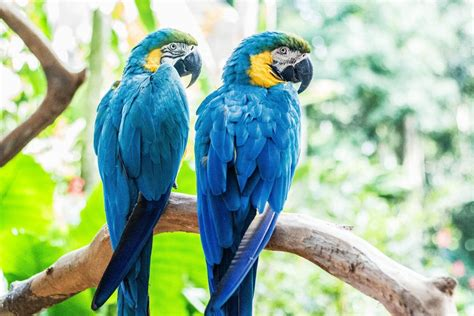
\includegraphics[width=.5\textwidth]{imagem/arara1.jpg}
        \label{fig:casal-araras}
        \fonte{\textcite{carroll_2018}}
    \end{figure}
    
    \begin{table}[htbp]
      \centering
      \caption{Teste de tabela}
        \begin{tabular}{ccccc}
        \toprule
        Nome  & Descrição & E (m)     & N (m)    & h (m) \\
        \midrule
        1     & TESTE & 300000.000 & 7500000.000 & 1200.000 \\
        2     & TESTE & 300000.000 & 7500000.000 & 1200.000 \\
        3     & TESTE & 300000.000 & 7500000.000 & 1200.000 \\
        4     & TESTE & 300000.000 & 7500000.000 & 1200.000 \\
        \bottomrule
        \end{tabular}%
      \label{tab:tabela-teste} % permite citar corretamente a tabela.
      \fonte{\textcite{carroll_2018}}
    \end{table}%


    
% ----------------------------------------------------------


    
% ----------------------------------------------------------
\chapter{CAPÍTULO 3}

    \lipsum[4]
    
    \begin{figure}[htpb]
        \centering
        \caption{Tucano.}
        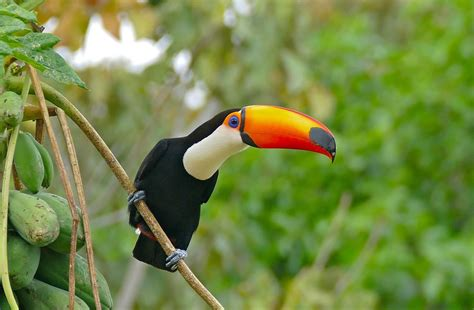
\includegraphics[width=.5\textwidth]{imagem/tucano.jpg}
        \label{fig:tucano}
        \fonte{COLOQUE A FONTE.}
    \end{figure}

    \lipsum[5]

% ----------------------------------------------------------
% ELEMENTOS PÓS-TEXTUAIS
% ----------------------------------------------------------
\postextual

% ----------------------------------------------------------
% Referências bibliográficas
% ----------------------------------------------------------

%biblatex-abnt do Daniel
\printbibliography[title={REFERÊNCIAS}] % para inserir o nome das referências em maiúsculo.

% ----------------------------------------------------------
% Apêndices
% ----------------------------------------------------------

% ---
% Inicia os apêndices
% ---
%\begin{apendicesenv}

% Imprime uma página indicando o início dos apêndices
% \partapendices

% ----------------------------------------------------------
%\chapter{EXEMPLO DE APÊNDICE}

%\end{apendicesenv}
% ---


% ----------------------------------------------------------
% Anexos
% ----------------------------------------------------------

% ---
% Inicia os anexos
% ---
%\begin{anexosenv}

% Imprime uma página indicando o início dos anexos
%\partanexos

%\chapter{SE PRECISAR DOS ANEXOS}

%\end{anexosenv}

\end{document}